\section{Kết quả thống kê mô tả}
Câu hỏi mô tả đặt ra là các đặc trưng lưu lượng có xu hướng trung tâm, mức phân tán và hình dạng phân bố như thế nào trong KDDTrain+ ($n=125.973$). Sáu biến đại diện được chọn theo ý nghĩa đo lường: \texttt{duration} phản ánh thời lượng kết nối; \texttt{src\_bytes} và \texttt{dst\_bytes} phản ánh lượng dữ liệu hai chiều; \texttt{count} và \texttt{srv\_count} thể hiện số kết nối trong cửa sổ hai giây, lần lượt tới cùng máy đích và cùng dịch vụ; \texttt{serror\_rate} là tỷ lệ lỗi SYN trong các kết nối cùng máy đích \cite{task2_kdd1999}. Lựa chọn này bao quát thời gian, lưu lượng, hoạt động kết nối và lỗi giao thức, không dựa trên kết quả của Test.

Bảng~\ref{tab:t2:descriptive} trình bày trung bình, trung vị, độ lệch chuẩn và cực trị. Bảng~\ref{tab:t2:quantiles} bổ sung các phân vị và tỷ lệ bằng 0 để đánh giá mức độ trung bình đại diện cho quan sát điển hình. Phương sai và độ lệch chuẩn mẫu dùng mẫu số $n-1$; phân vị sử dụng nội suy tuyến tính tại vị trí $(n-1)p$ trong dãy đã sắp xếp (chỉ số bắt đầu từ 0). Các đặc trưng đều có đủ $n$ quan sát.
\begin{table}[H]
\centering
\caption{Xu hướng trung tâm và độ phân tán trên KDDTrain+ ($n=125.973$ cho mỗi biến)}
\label{tab:t2:descriptive}
\small
\setlength{\tabcolsep}{3pt}
\begin{tabular}{lrrrrr}
\toprule
Đặc trưng & Trung bình & Trung vị & ĐLC mẫu & Min & Max \\
\midrule
\texttt{duration} & 287,14 & 0,00 & 2.604,52 & 0 & 42.908 \\
\texttt{src\_bytes} & 45.566,74 & 44,00 & 5.870.331,18 & 0 & 1.380e09 \\
\texttt{dst\_bytes} & 19.779,11 & 0,00 & 4.021.269,15 & 0 & 1.310e09 \\
\texttt{count} & 84,11 & 14,00 & 114,51 & 0 & 511 \\
\texttt{srv\_count} & 27,74 & 8,00 & 72,64 & 0 & 511 \\
\texttt{serror\_rate} & 0,284 & 0,000 & 0,446 & 0 & 1 \\
\bottomrule
\end{tabular}
\par\smallskip\footnotesize \texttt{duration}: giây; \texttt{src\_bytes}, \texttt{dst\_bytes}: byte; \texttt{count}, \texttt{srv\_count}: số kết nối; \texttt{serror\_rate}: tỷ lệ 0--1. Ký hiệu eN nghĩa là nhân $10^N$.
\end{table}\begin{table}[H]
\centering
\caption{Phân vị, phương sai mẫu và tỷ lệ bằng 0 trên KDDTrain+}
\label{tab:t2:quantiles}
\small
\setlength{\tabcolsep}{3pt}
\begin{tabular}{lrrrrr}
\toprule
Đặc trưng & $Q_1$ & $Q_3$ & IQR & Phương sai mẫu & Bằng 0 (\%) \\
\midrule
\texttt{duration} & 0 & 0 & 0 & 6.783.500,00 & 92,05 \\
\texttt{src\_bytes} & 0 & 276 & 276 & 3.446e13 & 39,21 \\
\texttt{dst\_bytes} & 0 & 516 & 516 & 1.617e13 & 53,95 \\
\texttt{count} & 2 & 143 & 141 & 13.112,22 & 0,01 \\
\texttt{srv\_count} & 2 & 18 & 16 & 5.275,97 & 0,01 \\
\texttt{serror\_rate} & 0 & 1 & 1 & 0,199 & 68,93 \\
\bottomrule
\end{tabular}
\par\smallskip\footnotesize Phương sai có đơn vị bình phương: giây$^2$, byte$^2$, kết nối$^2$; phương sai của tỷ lệ không có đơn vị vật lý. IQR giữ đơn vị gốc.
\end{table}
Thời lượng có trung vị 0 giây và 92,05\% quan sát bằng 0, trong khi trung bình là 287,14 giây và cực đại 42.908 giây. Số 0 là giá trị được ghi ở độ phân giải giây, không nhất thiết có nghĩa không tồn tại kết nối. Việc các phân vị 25\%, 50\% và 75\% cùng bằng 0 cho thấy trung bình bị chi phối bởi phần nhỏ quan sát có thời lượng lớn; chỉ báo này cần được đọc cùng phân vị thay vì xem như thời lượng điển hình.

Hai biến byte đều lệch mạnh về phía giá trị lớn. Với \texttt{src\_bytes}, trung bình 45.566,74 byte vượt xa trung vị 44 byte, còn độ lệch chuẩn đạt 5.870.331,18 byte. Với \texttt{dst\_bytes}, hơn một nửa quan sát bằng 0 (53,95\%), dù trung bình đạt 19.779,11 byte. Các cực trị rất lớn làm phương sai tăng mạnh, nhưng chỉ từ bảng mô tả, nghiên cứu chưa xác định được các cực trị này là lỗi ghi nhận hay phản ánh hành vi mạng đặc thù.

\texttt{count} có trung bình 84,11 và trung vị 14 kết nối, cao hơn các chỉ tiêu tương ứng của \texttt{srv\_count} (27,74 và 8). Hai biến sử dụng điều kiện đếm khác nhau nên không được suy ra quan hệ tập con từ chênh lệch này. \texttt{serror\_rate} có trung vị 0 nhưng $Q_3=1$, cho thấy đồng thời có nhiều quan sát không có lỗi SYN và một phần đáng kể ở tỷ lệ lỗi cao. Đặc điểm này là cơ sở để nghiên cứu tiếp tục xem xét phân bố theo nhãn, bên cạnh trung bình toàn mẫu.
\FloatBarrier

\section{Phân bố nhãn và so sánh đặc trưng Normal/Attack}
Bảng~\ref{tab:t2:labels} và Hình~\ref{fig:t2:labels} cho thấy cơ cấu gồm Normal và bốn nhóm tấn công. Normal chiếm 53,458\%, Attack chiếm 46,542\%; tuy hai nhãn nhị phân có quy mô tương đối gần nhau, cơ cấu bên trong Attack mất cân bằng rõ rệt. DoS có 45.927 quan sát, còn R2L chỉ có 995 và U2R chỉ có 52. Vì vậy, sự cân đối tương đối của bài toán nhị phân không đồng nghĩa năm nhóm đều có số quan sát tương tự.
\begin{table}[H]
\centering
\caption{Phân bố năm nhóm và tổng hợp nhị phân trên KDDTrain+}
\label{tab:t2:labels}
\small
\setlength{\tabcolsep}{3pt}
\begin{tabular}{lrr}
\toprule
Nhãn & Tần số & Tỷ lệ (\%) \\
\midrule
Normal & 67.343 & 53,458 \\
DoS & 45.927 & 36,458 \\
Probe & 11.656 & 9,253 \\
R2L & 995 & 0,790 \\
U2R & 52 & 0,041 \\
\midrule Tổng & 125.973 & 100,000 \\
\midrule Normal (nhị phân) & 67.343 & 53,458 \\
Attack (nhị phân) & 58.630 & 46,542 \\
\bottomrule
\end{tabular}
\par\smallskip\footnotesize Attack là tổng DoS, Probe, R2L và U2R; hai hàng nhị phân là cách gộp lại cùng mẫu, không cộng thêm vào tổng năm nhóm.
\end{table}\begin{figure}[H]
\centering
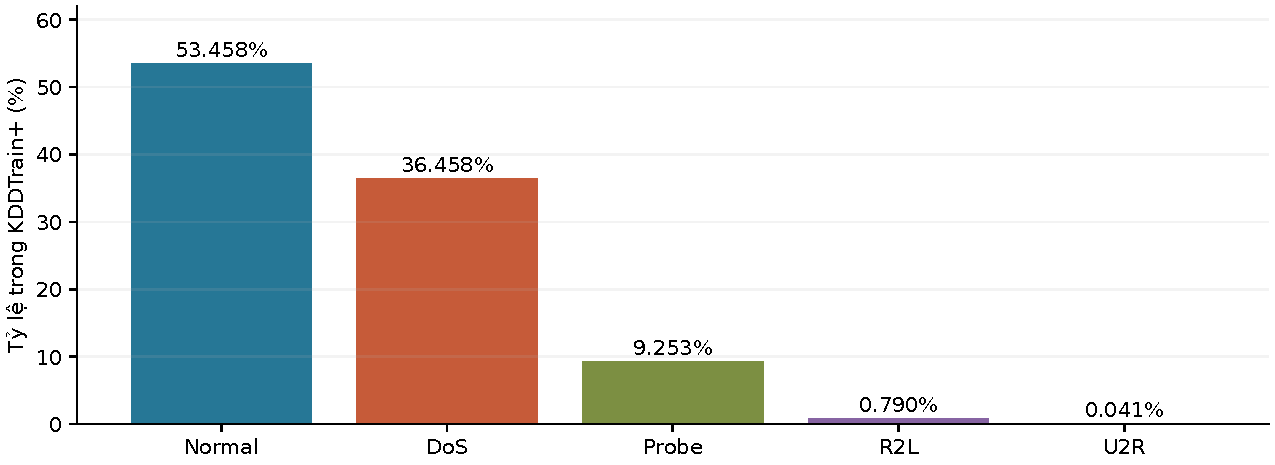
\includegraphics[width=1.0\linewidth]{figures/task2_labels.pdf}
\caption{Tỷ lệ Normal và bốn nhóm tấn công trên KDDTrain+ ($n=125.973$). Trục tung tuyến tính; giá trị ghi trên cột giúp nhận biết hai nhóm hiếm.}
\label{fig:t2:labels}
\end{figure}
Tỷ lệ DoS cao khiến các đặc điểm của nhóm tấn công này có thể chi phối kết quả gộp Attack. R2L và U2R có số quan sát nhỏ nên kết quả mô tả Attack không được xem là mô tả riêng cho hai nhóm đó. Các tỷ lệ ở Bảng~\ref{tab:t2:labels} phản ánh thành phần mẫu được cung cấp, không phản ánh xác suất gặp tấn công trong mạng đang vận hành.

Để so sánh hai nhãn, ba đặc trưng được chọn vì có cơ chế diễn giải bổ sung nhau: \texttt{src\_bytes} đo dữ liệu truyền từ nguồn, \texttt{count} đo mức tập trung kết nối tới máy đích trong hai giây, còn \texttt{serror\_rate} phản ánh lỗi SYN. Bảng~\ref{tab:t2:comparison} so sánh trực tiếp hai nhóm, còn Hình~\ref{fig:t2:histograms} mô tả toàn bộ phân bố và Hình~\ref{fig:t2:boxplots} nhấn mạnh trung vị, khoảng tứ phân vị và các điểm xa hộp.
\begin{table}[H]
\centering
\caption{So sánh trực tiếp Normal và Attack trên KDDTrain+}
\label{tab:t2:comparison}
\small
\setlength{\tabcolsep}{3pt}
\begin{tabular}{llrrrr}
\toprule
Đặc trưng & Nhóm ($n$) & TB & Trung vị & ĐLC mẫu & $Q_1$--$Q_3$ \\
\midrule
\texttt{src\_bytes} & Normal (67.343) & 13.133,28 & 233 & 418.113,13 & 129--324 \\
\texttt{src\_bytes} & Attack (58.630) & 82.820,14 & 0 & 8.593.024,60 & 0--0 \\
\texttt{count} & Normal (67.343) & 22,52 & 4 & 54,03 & 1--14 \\
\texttt{count} & Attack (58.630) & 154,85 & 138 & 124,33 & 40--241 \\
\texttt{serror\_rate} & Normal (67.343) & 0,013 & 0 & 0,094 & 0--0 \\
\texttt{serror\_rate} & Attack (58.630) & 0,596 & 1 & 0,487 & 0--1 \\
\bottomrule
\end{tabular}
\par\smallskip\footnotesize TB: trung bình; ĐLC: độ lệch chuẩn. \texttt{src\_bytes}: byte; \texttt{count}: kết nối; \texttt{serror\_rate}: tỷ lệ 0--1. Tính trên dữ liệu gốc, không logarit hóa.
\end{table}
Trung vị \texttt{count} ở Attack là 138, so với 4 ở Normal, tức cao hơn 134 kết nối; khoảng tứ phân vị tương ứng là 40--241 và 1--14. Điều này phù hợp với một số hành vi tạo nhiều kết nối trong thời gian ngắn như từ chối dịch vụ hoặc thăm dò. Tuy nhiên, cả hai nhóm đều có giá trị từ 0 đến 511, nên miền giá trị vẫn chồng lấp và không thể dùng riêng số kết nối để nhận diện mọi cuộc tấn công.

Với \texttt{serror\_rate}, trung bình Attack là 0,596, so với 0,013 ở Normal; trung vị lần lượt là 1 và 0. Mặc dù lỗi SYN tập trung rõ hơn trong Attack, 36,99\% quan sát Attack vẫn có tỷ lệ lỗi bằng 0, còn 3,27\% Normal có tỷ lệ lỗi dương. Sự chồng lấp quan sát được này cho thấy ngưỡng có lỗi/không lỗi sẽ bỏ sót một phần tấn công và gắn cờ một phần kết nối bình thường.
\begin{figure}[H]
\centering
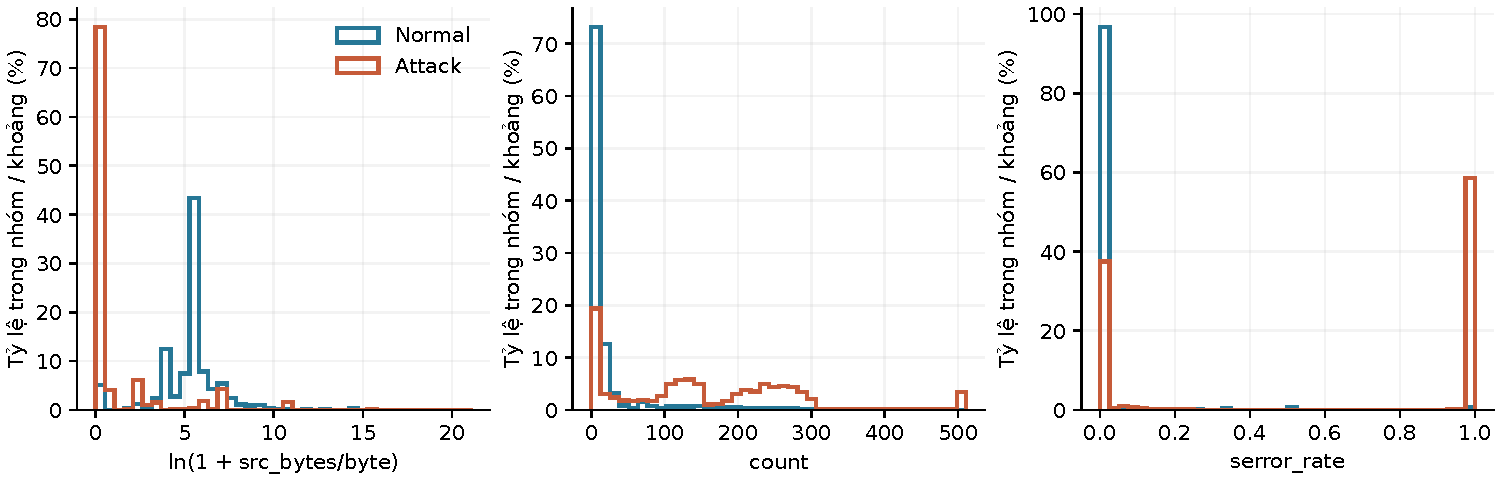
\includegraphics[width=1.0\linewidth]{figures/task2_histograms.pdf}
\caption{Histogram so sánh trên KDDTrain+: mỗi nhóm được chuẩn hóa riêng để tổng chiều cao các khoảng bằng 100\%; dùng cùng 40 khoảng chia đều cho hai nhóm ở từng ô. \texttt{src\_bytes} chỉ đổi thang trực quan thành $\ln(1+x/\mathrm{byte})$; hai biến còn lại giữ thang gốc. Không cắt miền giá trị.}
\label{fig:t2:histograms}
\end{figure}
Histogram cho thấy khác biệt của \texttt{src\_bytes} không thể tóm tắt bằng trung bình: Attack có trung bình 82.820,14 byte, cao hơn Normal (13.133,28 byte), nhưng trung vị Attack bằng 0, thấp hơn Normal (233 byte). Trong Attack, 78,42\% giá trị bằng 0, so với 5,07\% ở Normal. Phân bố vì vậy vừa có khối lượng lớn tại 0 vừa có đuôi phải rất dài. Trung bình cao không có nghĩa một kết nối Attack điển hình truyền nhiều byte hơn.
\begin{figure}[H]
\centering
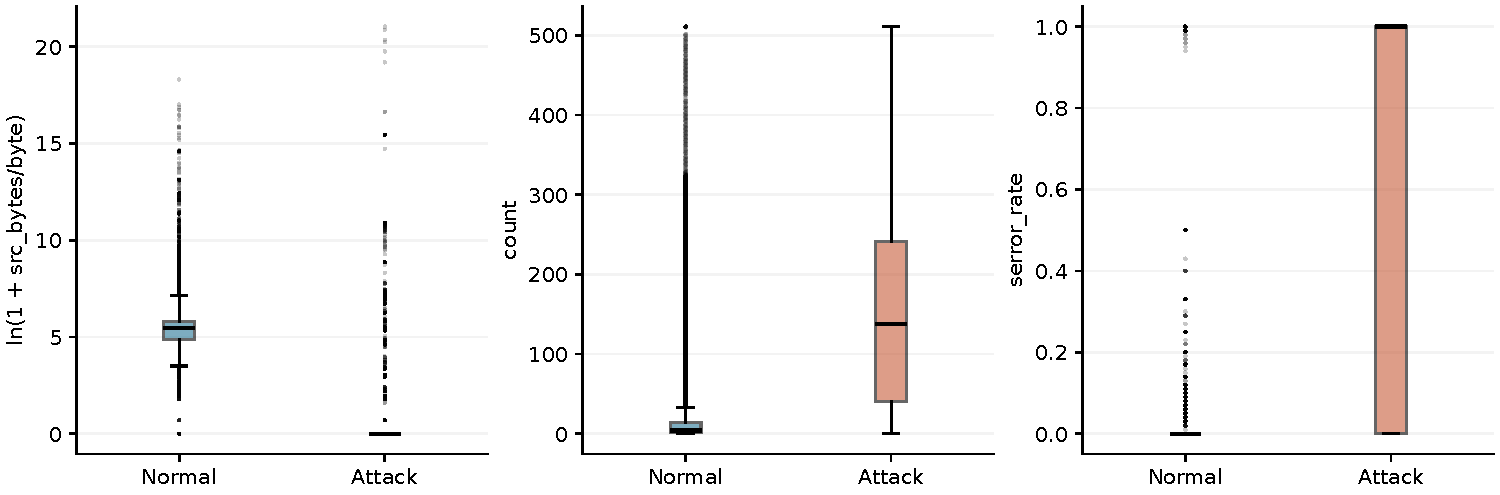
\includegraphics[width=1.0\linewidth]{figures/task2_boxplots.pdf}
\caption{Boxplot theo nhãn trên KDDTrain+. Hộp biểu diễn $Q_1$--$Q_3$, đường giữa là trung vị; râu tới quan sát xa nhất còn trong ngưỡng $1{,}5\,IQR$ trên thang vẽ; các điểm ngoài râu vẫn được hiển thị. Chỉ \texttt{src\_bytes} dùng $\ln(1+x/\mathrm{byte})$, giữ toàn bộ miền.}
\label{fig:t2:boxplots}
\end{figure}
Boxplot làm nổi bật khoảng tứ phân vị của \texttt{count} ở Attack dịch lên cao. Tuy nhiên, hộp \texttt{src\_bytes} của Attack co lại ở 0 do $Q_1=Q_3=0$; hộp \texttt{serror\_rate} của Normal cũng co tại 0. Khi IQR bằng 0, các điểm ngoài hộp không tự động là dữ liệu sai. Phép logarit giúp nhìn phần đuôi của biến byte nhưng không làm biến mất sự chồng lấp giữa hai nhãn. Các khác biệt nêu trên chỉ là kết quả mô tả, chưa xác lập ý nghĩa thống kê, quan hệ nhân quả hay hiệu quả dự đoán.
\FloatBarrier

